\documentclass{sig-alternate-05-2015}
\usepackage{graphicx}
\graphicspath{{img/}}
\usepackage{hyperref}
\usepackage{xcolor}
\definecolor{linkcolor}{HTML}{799B03} % цвет ссылок
\definecolor{urlcolor}{HTML}{799B03} % цвет гиперссылок
\begin{document}

\title{Hotel Management System}
\subtitle{\href{https://andrew_it@bitbucket.org/andrew_it/hotel.git}{https://andrew\_it@bitbucket.org/andrew\_it/hotel.git}}


\numberofauthors{2}
\author{
\alignauthor
Ermak Andrey\\
       \affaddr{Innopolis, Russia}\\
       \email{79174358525@ya.ru}
\alignauthor
Khizilov Mikhail\\
	   \affaddr{Innopolis, Russia}\\
       \email{email}
}

\date{17 October 2017}

\maketitle

\section{Tasks}
In this project we need to implement a hotel management system, like booking.com in mobile-friendly web interface. 

In ours project we have several feacues:

\begin{enumerate}
\item Mobile-friendly design
\item Searching hotel by Country/City/Name in one field. Searching constrainted by check-in and check-out date
\item Advanced searching with some parameters, such as wi-fi, tv, bathroom etc. 
\item Registration hotels owners and users
\item Hotel manager's features
\begin{enumerate}
	\item You can add, managed and delete your own hotel
	\item All hotels have own image
	\item Every hotel have rooms and receptionists to manage
	\item Receptionist can manage all booking in the hotel
\end{enumerate}
\item User's features
\begin{enumerate}
	\item You can change your profile
	\item You can booked and manage your bookings
\end{enumerate}
\end{enumerate}

There is the distribution of the roles:\\
Andrey: Front-end, Data generation, DB management\\
Mikhail: Back-end, DB management\\
Common: ER-dyagram, normalization of DB


\section{System Design and Architecture}
There is 12 tables in our project:
\begin{enumerate} 	
\item country(\underline{country}, \underline{city})
\item sys\_user(\underline{user\_id}, email, password, role)
\item hotel\_admin(\underline{user\_id}, first\_name, last\_name, phone\_number)
\item hotel(\underline{hotel\_id}, city, address, name, stars, description, img, owner\_id)
\item room\_condig(\underline{config\_id}, single\_bed, double\_bed, sofa\_bed)
\item customer(\underline{person\_id}, first\_name,  last\_name, phone\_number, payment\_info)
\item admin(\underline{person\_id}, first\_name,  last\_name, phone\_number)
\item receptionist(\underline{person\_id}, first\_name,  last\_name, phone\_number, salary)
\item transaction(\underline{transaction\_id}, customer\_id, payment\_method, amount)
\item room\_option(\underline{option\_id}, is\_bathroom, is\_tv, is\_wifi, is\_bathhub, is\_airconditioniring)
\item room(\underline{room\_id}, hotel\_id, config\_id, option\_id, quantity, title, description, cost)
\item booking(\underline{room\_id}, \underline{customer\_id}, \underline{transaction\_id}, quantity, checkin\_idate, checkout\_date)
\end{enumerate}

There is cool feature in table "room\_config": this table consists of all combinations of (double bed, single bed, sofa) represented in any hotels in the site. In fact, there is very small table which can describe most of room configurations in all hotels at the site. 

Table "room\_option" has the same feature, but there is a only boolean fields - this means the maximum size of table is $ 2^x $, where $x$ - number of options.

There is several tables with same fields: "hotel\_admin", "customer", "admin", "receptionist". There is for physical independence. 



\section{The application}
In ours project we used the following stack of technologies:
\begin{enumerate}
	\item PostgreSQL - one of the best relation databases
	\item Flask - is a microframework for Python based on Werkzeug, Jinja 2 and good intentions. 
	\item Bootstrap - is the most popular HTML, CSS, and JS framework for developing responsive, mobile first projects on the web.
\end{enumerate}

Flask consists of many parts, such as:
\begin{enumerate}
	\item Flask-Bcrypt -- library for creating and veryficating passwords
	\item Flask-Login -- library for creating and storing session
	\item Flask-WTF -- library for usefull creation and and communication with html-pages
\end{enumerate}

For connecting to database, we uses non-ORM library psycopg2

{The SQL commands used to obtain the statistics}
This is SQL which show perfomance od DB:
\begin{verbatim}
	SELECT blks_hit::float/(blks_read + blks_hit) as 
	cache_hit_ratio, numbackends 
	FROM pg_stat_database WHERE datname='hms'
\end{verbatim}
There some SQL views:
\begin{verbatim}
CREATE VIEW vw_hotels AS
SELECT *
FROM hotel JOIN country USING (city);

CREATE VIEW vw_customers AS
SELECT person_id, first_name, last_name, 
phone_number, payment_info, email
FROM sys_user JOIN customer ON (user_id=person_id);

CREATE VIEW vw_booked_rooms AS
SELECT  room_id, hotel_id, title, r.config_id, 
r.option_id, description, cost,
b.quantity, checkin_date, checkout_date,
single_bed, double_bed, sofa_bed,
is_bathroom, is_tv, is_wifi, is_bathhub, 
is_airconditioniring,
first_name, last_name, phone_number
FROM room r JOIN booking b USING (room_id)
JOIN room_config rc USING (config_id)
JOIN room_option ro USING (option_id)
JOIN customer c ON (c.person_id=b.customer_id);
\end{verbatim}
There is one of biggest quiry of the application:
\begin{verbatim}
SELECT * FROM hotel h INNER JOIN country c 
ON (h.city=c.city) AND
 (lower(h.city) LIKE %(destination)s OR 
 lower(c.country) LIKE %(destination)s OR 
 lower(h.name) LIKE %(destination)s) AND 
 EXISTS(SELECT r.hotel_id FROM room r 
 INNER JOIN room_config rc ON 
 (r.config_id=rc.config_id) WHERE
  r.quantity > (SELECT coalesce(MAX(b.quantity), 0) 
 FROM booking b WHERE r.room_id = b.room_id AND 
 NOT (%(checkout)s <= b.checkin_date 
 OR %(checkin)s >= b.checkout_date)) 
 AND r.quantity >= %(quantity)s AND 
 (rc.single_bed + 2 * rc.double_bed + 
 rc.sofa_bed >= %(sleeps)s)
\end{verbatim}

\subsection{Highlight specific novel ideas that your team has used in the application}
There is some features in our project:
\begin{enumerate}
	\item Tables "room\_config" and "room\_options"
	\item There is the ability to insert the pictures to hotels
	\item Python script for generating data
	\item Mobile friendly
	\item Managing and editing hotels
	\item Template-based creating html-pages
	\item The unified field of the login for all types of users
	\item The unified field of the searching hotels
	\item BCNF
\end{enumerate}
\subsubsection{Tables "room\_config" and "room\_options"}
This tables -- is really cool idea, we don't write any options or config inside 'room' tuple - we only have two references to tables "room\_config" and "room\_options" which store all combination of options/config's in this site. This is allow to safe a lot of disk space, because we only store $ 2^x $combinations in "room\_options", where $x$ - number of options and $ single_bed*double_bed*sofa $ combinations of configs instead millions redundant cells.

\subsubsection{There is the ability to insert the pictures to hotels}
All hotels have custom image file, which you can upload on your hotel

\subsubsection{Python script for generating data}
Specially for this project, we write python-script, which randomly generate data in *.sql files.

\subsubsection{Mobile friendly}
This is mobile friendly web-site, due using bootstrap framework

\subsubsection{Managing and editing hotels}
If you hotel administrator, you able to manage and edit your hotel: you can create rooms, create and manage receptionists in your profile on site

\subsubsection{Template-based creating html-pages}
There is great technology in Flask -- templating, which help to dynamically create html-pages on server


\subsection{Insights of your learning during the course of doing the project}
\subsubsection{The unified field of the login for all types of users}
There is very useful, when you don't need to search special login form for your case -- sing-in and get your custom page!

\subsubsection{The unified field of the searching hotels}
There is really great search-field: You can search by Country/City/NameOfHotel in only one field. You only need to fill check-in, check-out and searching field and push "Search", or You can additionally use advanced searching by options, config's and costs. 

\subsubsection{BCNF}
All talbe in BD is in BCNF relation
\subsubsection{Admin perfomance panel}
The main admin of the site can see the performance of the site. Actually main admin can add the same admins with same access except access on deleting main admins

\subsection{Screenshots of the application}

\begin{figure*}[h]
	\begin{minipage}[h]{0.49\linewidth}
		\center{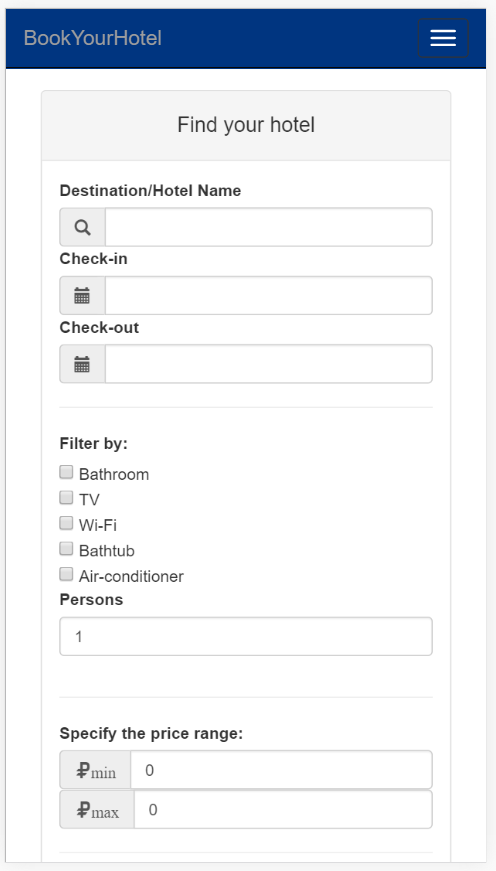
\includegraphics[width=1\linewidth]{search}}
	\end{minipage}
	\hfill
	\begin{minipage}[h]{0.49\linewidth}
		\center{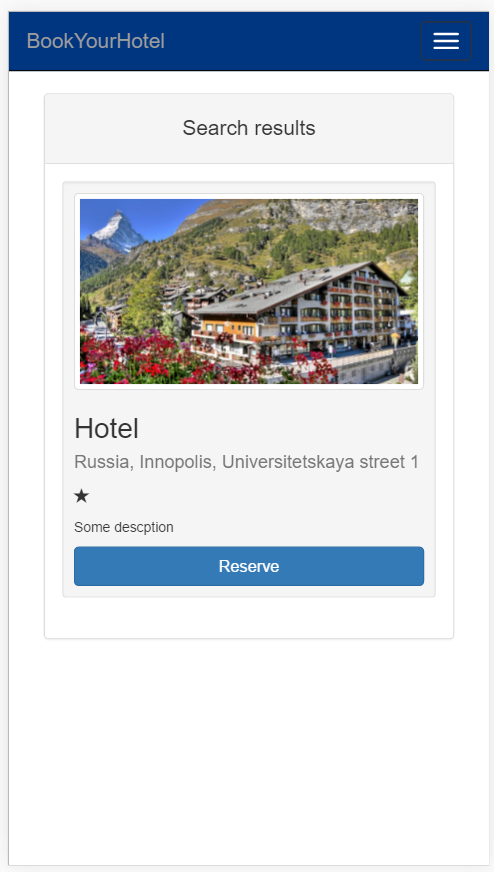
\includegraphics[width=1\linewidth]{result}}
	\end{minipage}
	\caption{(mobile)Searching and results}
	\label{search}
\end{figure*}
\begin{figure*}[h]
\centering
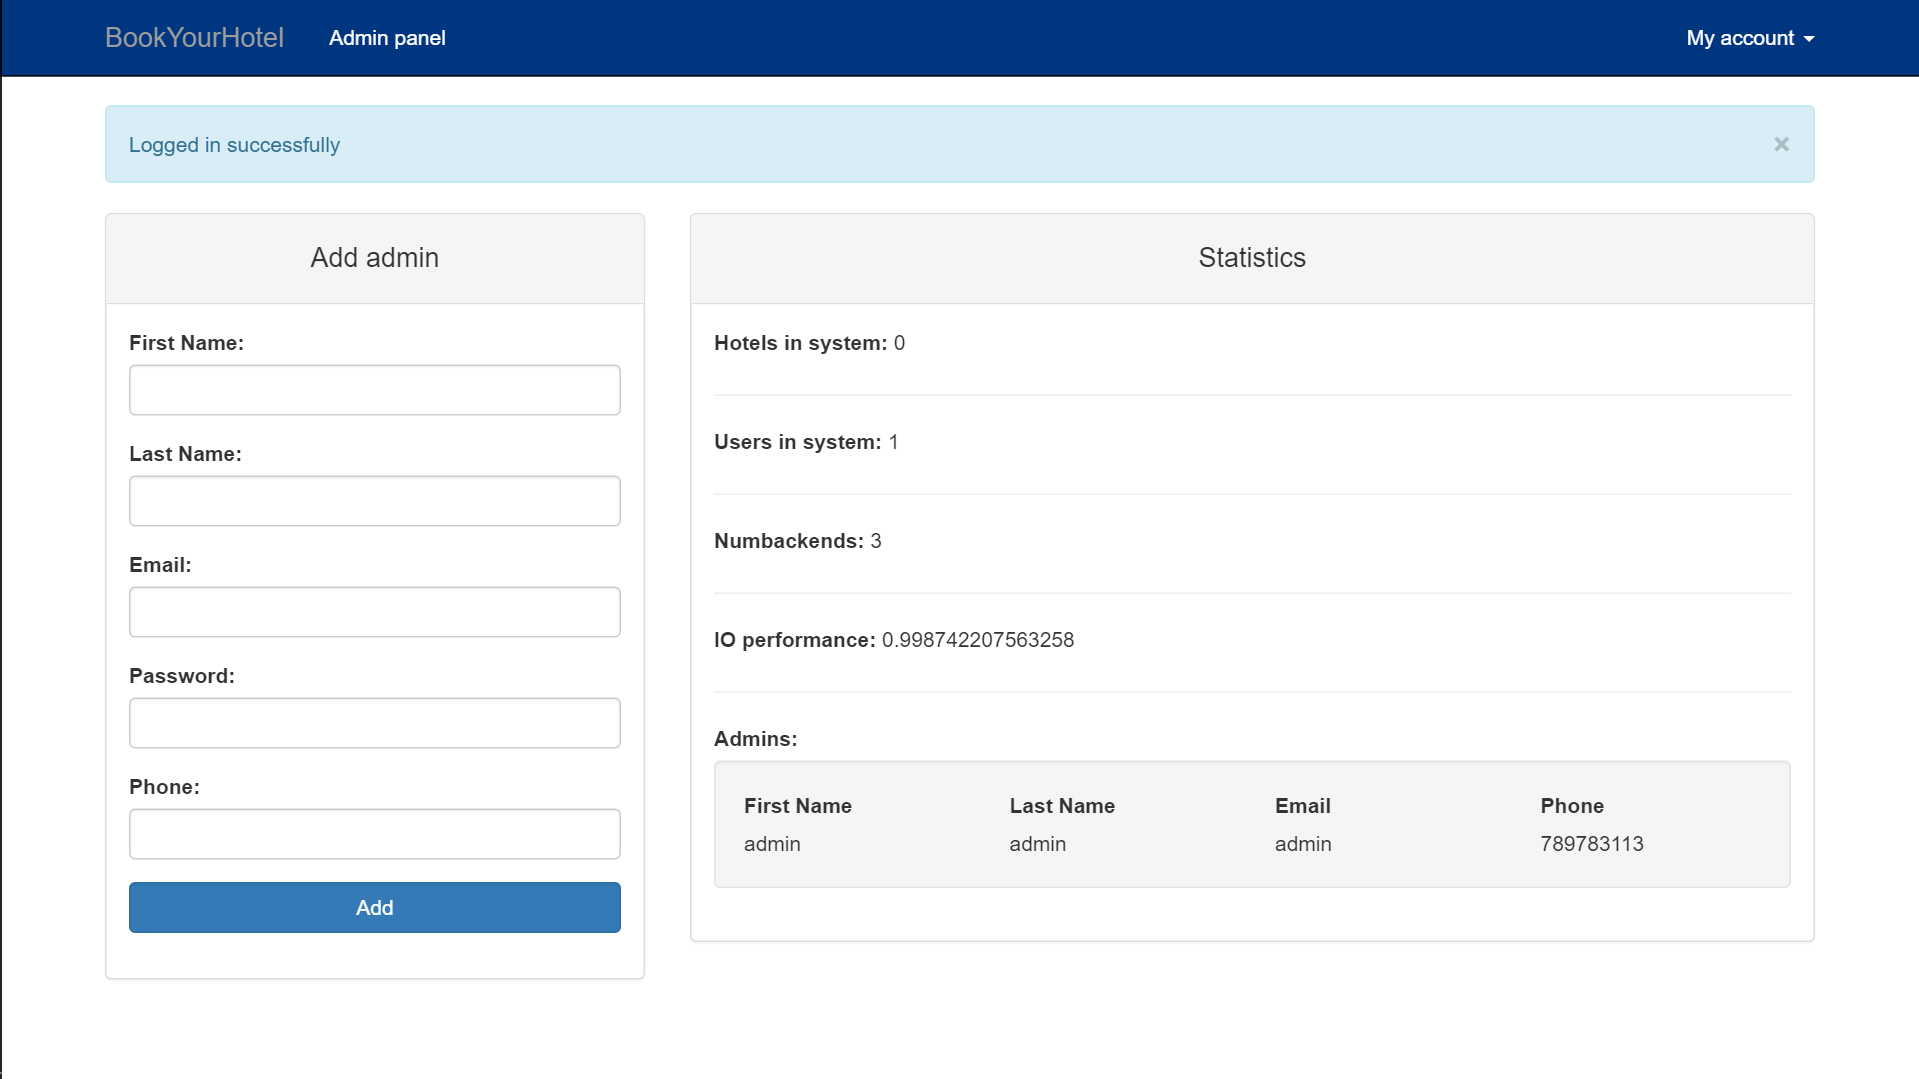
\includegraphics[width=1\linewidth]{adminpanel}
\caption{Admin panel}
\label{ap}
\end{figure*}
\begin{figure*}[h]
\centering
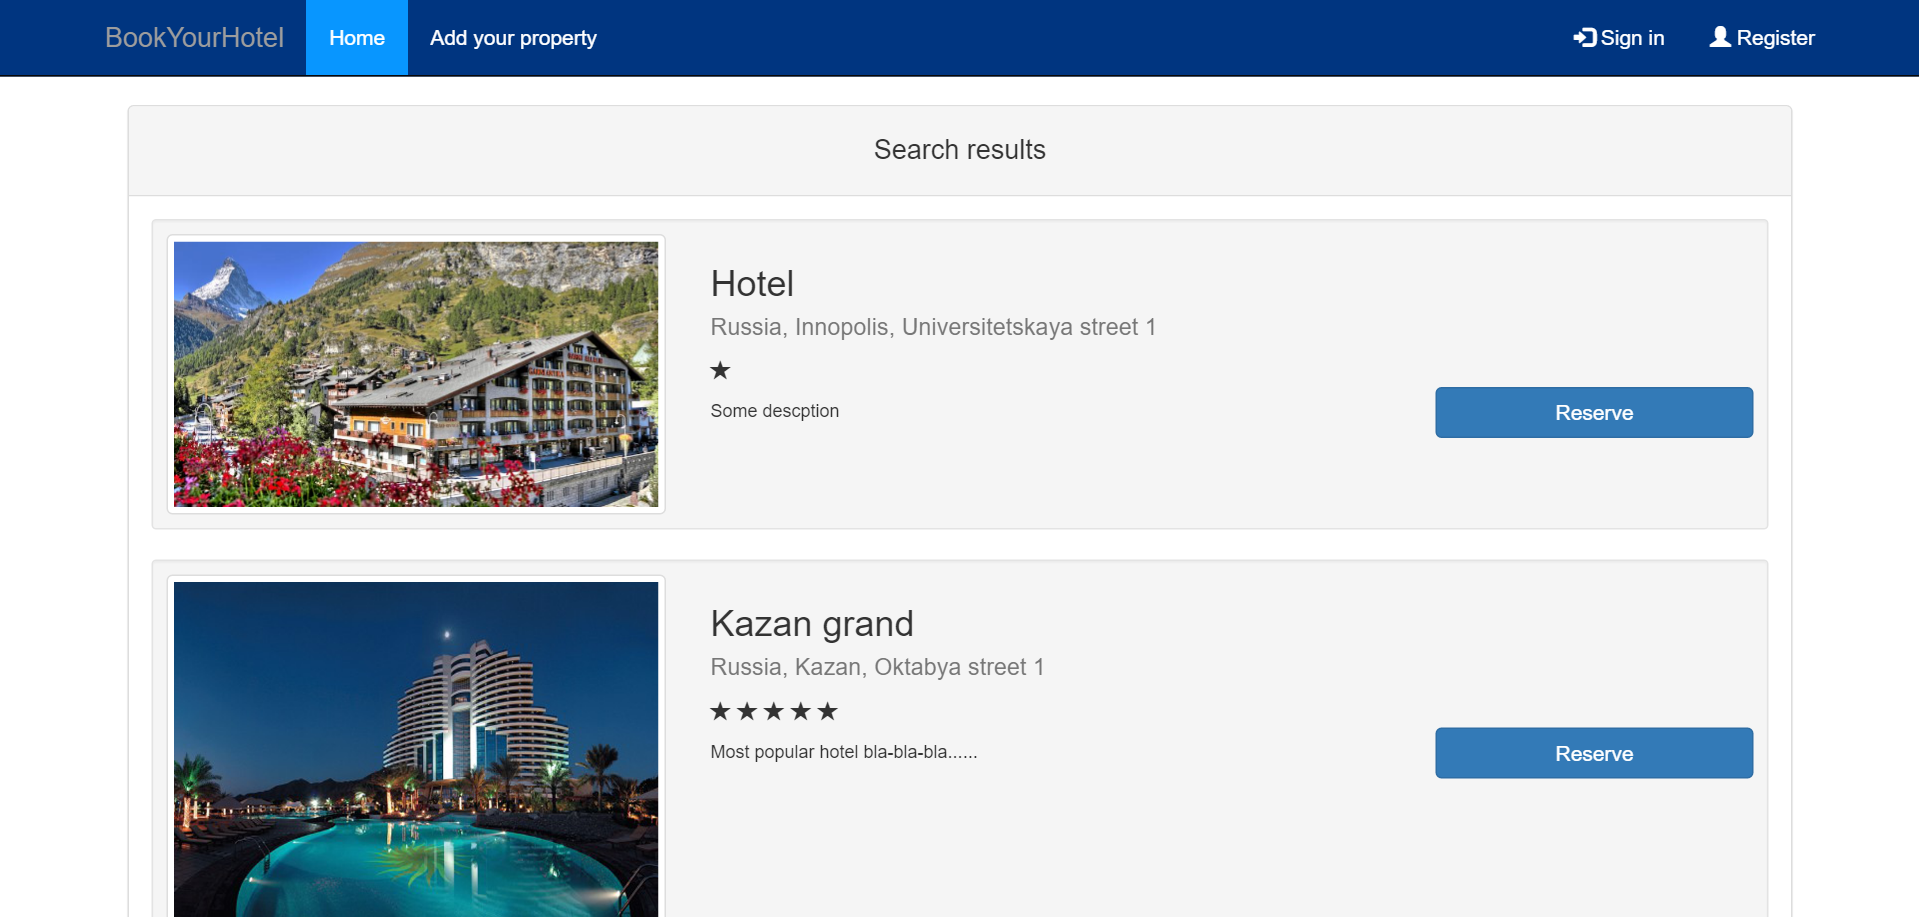
\includegraphics[width=1\linewidth]{reserve}
\caption{Reserve hotel}
\label{reserve}
\end{figure*}
\begin{figure*}[h]
	\centering
	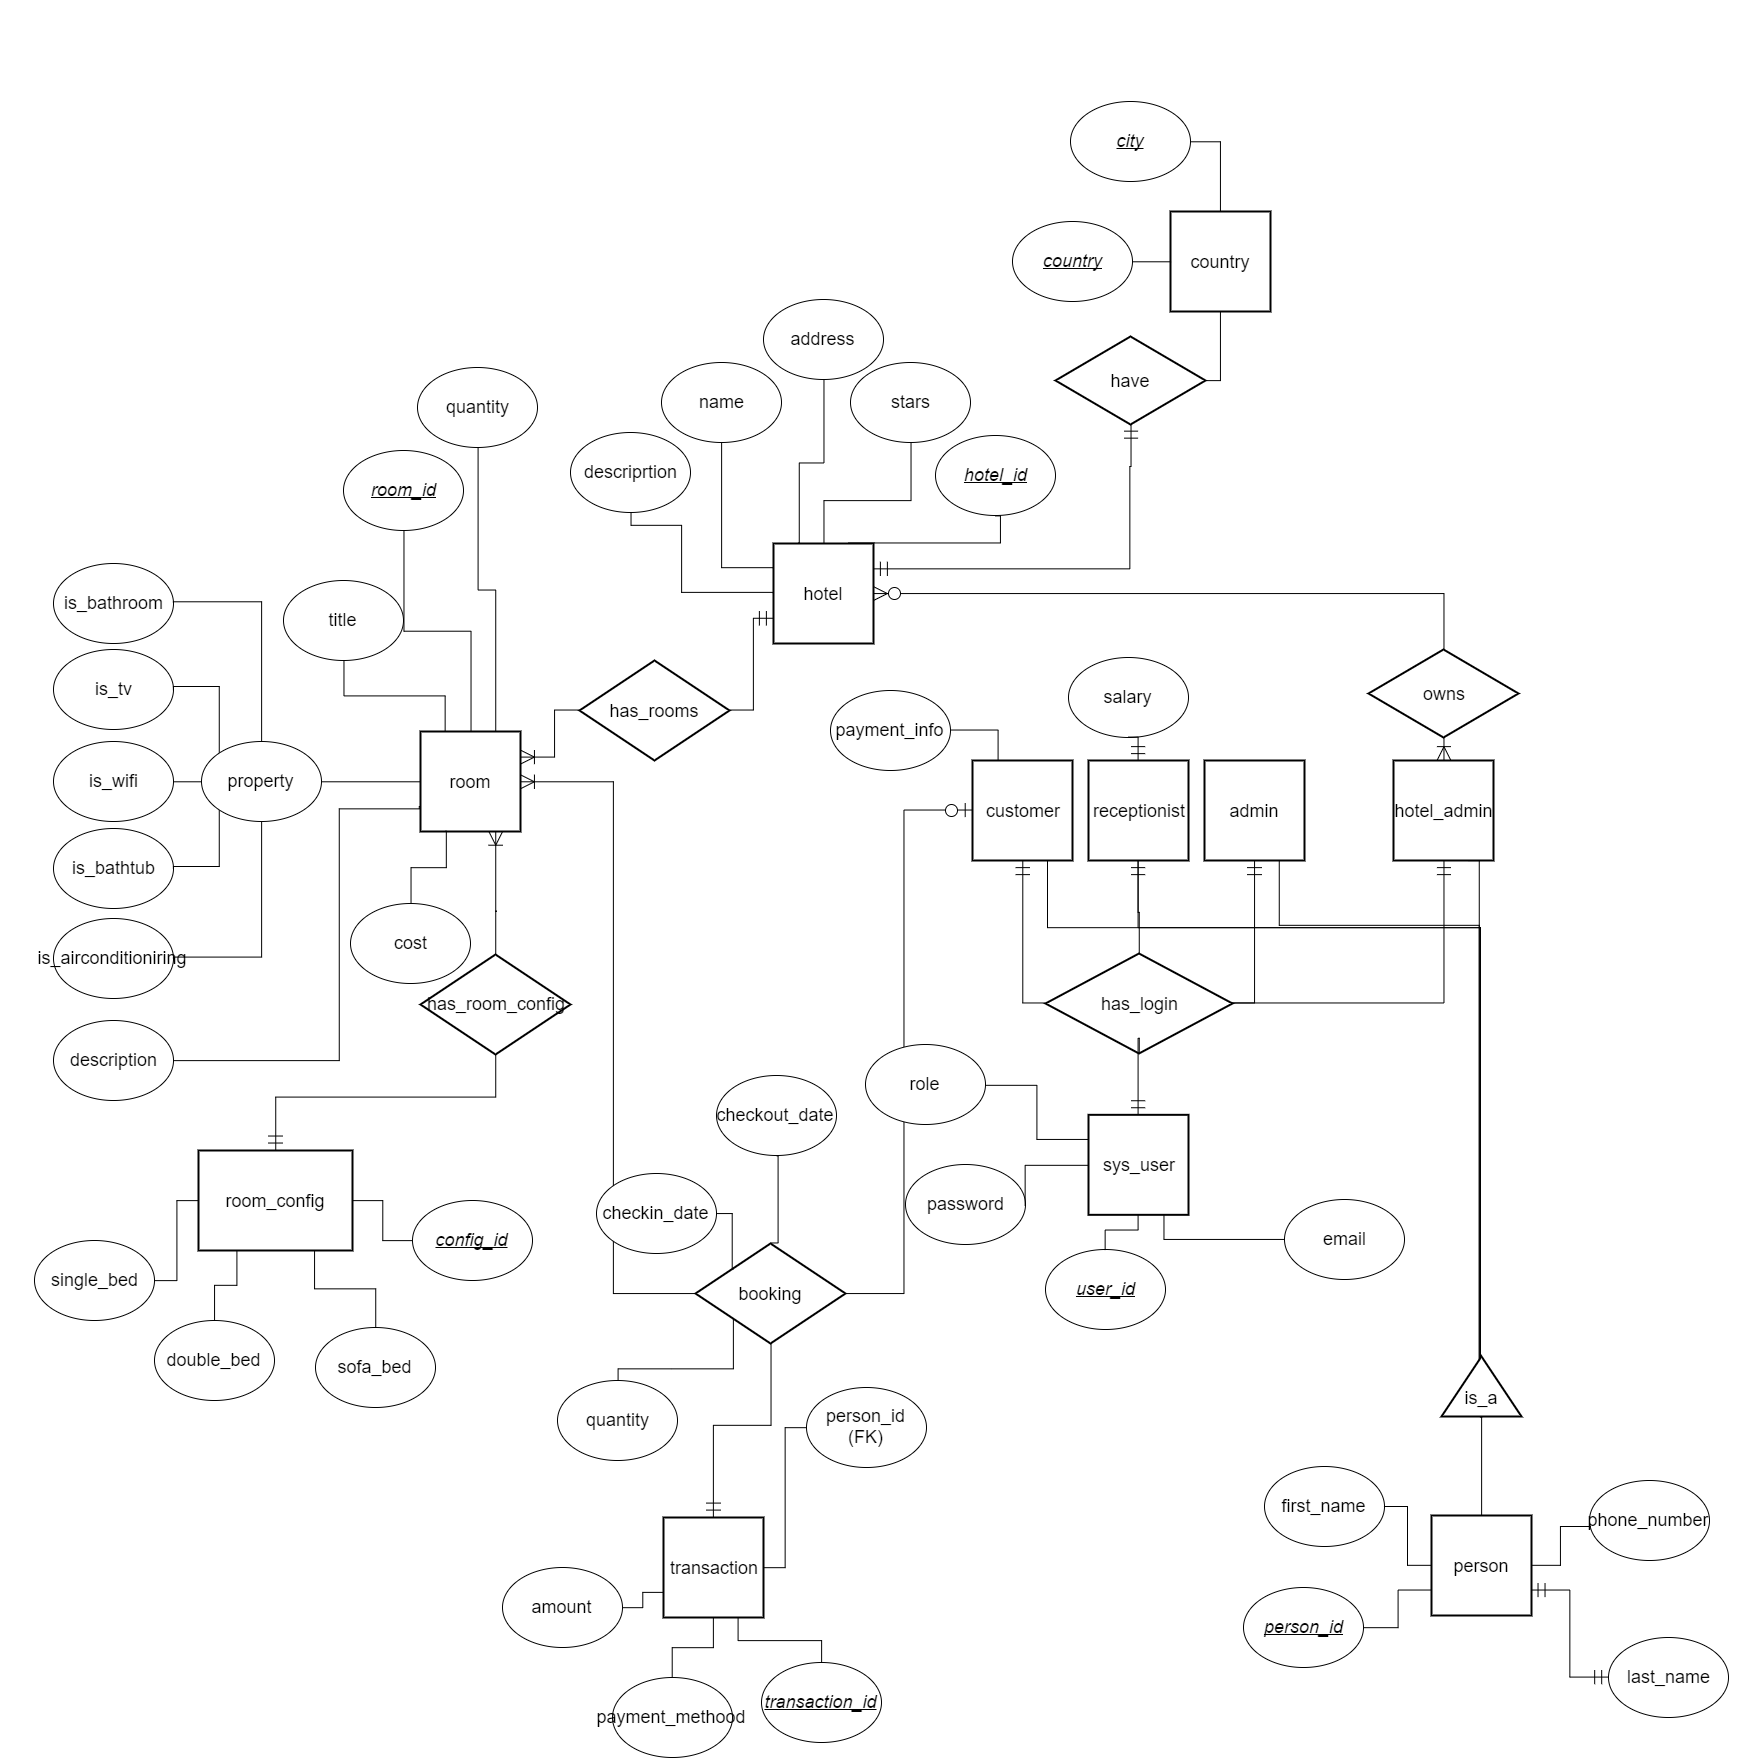
\includegraphics[width=1\linewidth]{er}
	\caption{ER diagram}
	\label{er}
\end{figure*}
\end{document}
